\subsection{Intégration numérique de $S$ et $T$}

\subsubsection{Intégration implicite de $S$}

\label{ssec:integration_S_imp}

L'intégration implicite revient à calculer $S^t$ en fonction de $S^{t+1}$, ce
qui donne un système linéaire qu'il est ensuite possible d'inverser. Il est
important de noter que cette méthode est plus coûteuse à chaque pas de temps
qu'une méthode explicite, car elle nécessite l'inversion d'une matrice. Dans la simulation,
on vérifie systématiquement que le temps de relaxation de $T$ est plus faible que le temps 
visqueux.

\paragraph{Linéarisation des équations}

On souhaite intégrer $S^\star$, la densité surfacique adimensionnée. L'équation
d'évolution est :

\begin{equation}
  \frac{\partial S^\star}{\partial t^\star} = \frac{1}{x^2}\frac{\partial^2}{\partial x^2}\left(\nu^\star S^\star\right)
\end{equation}

Pour alléger les notations, nous allons ommettre les étoiles dans les
développements prochains. L'équation s'écrit alors en passant aux variables
discrètes, au temps $t$ et à la case $1<n\leq n_\textrm{max}$

\begin{equation}
  \label{eq:S_discret_n}
  \frac{S^{t+1}_n - S^t_n}{\Delta t} = \frac{1}{x_n^2}\frac{\nu^t_{n+1}S^{t+1}_{n+1} - 2 \nu^t_nS^{t+1}_n + \nu^t_{n-1}S^{t+1}_{n-1}}{\Delta x^2}
\end{equation}

À l'intérieur du disque, la densité de matière est supposée nulle
($\nu^t_{0}S^{t+1}_{0} = 0$). Physiquement, il est en effet attendu qu'aucune
orbite keplerienne circulaire ne soit stable en dessous de l'ISCO
(\emph{\emph{I}nnermost \emph{S}table \emph{C}ircular \emph{O}rbit}), située en
$r = 3M$. En approximation, on suppose donc que la densité de matière y est
nulle.

\begin{equation}
  \label{eq:S_discret_1}
  \frac{S^{t+1}_1 - S^t_1}{\Delta t} = \frac{1}{x_1^2}\frac{\nu^t_{2}S^{t+1}_{2} - 2 \nu^t_1S^{t+1}_1}{\Delta x^2}
\end{equation}

Pour la case $n = n_\textrm{max} = N$, on a d'après \eqref{eq:nuS_n_is_null}:

\begin{equation}
  \frac{\nu^{t}_{N+1}S^{t+1}_{N+1} - \nu^{t}_NS^{t+1}_N}{\Delta x} = \dot{M}^\star_N
\end{equation}

Il faut noter que $\dot{M}^\star_N$ vaut initialement $1$. Pour simuler
l'arrivée de matière par l'extérieur du disque, cette quantité est incrémentée
au fur et à mesure de la simulation. Donc l'équation \eqref{eq:S_discret_n}
s'écrit en $N$:

\begin{equation}
  \label{eq:S_discret_N}
  \frac{S^{t+1}_N - S^t_N}{\Delta t} = \frac{1}{x_N^2}\frac{\Delta x - \nu^{t}_NS^{t+1}_N + \nu^{t}_{N-1}S^{t+1}_{N-1}}{\Delta x^2}
\end{equation}

\paragraph{Écriture matricielle}

On réécrit \eqref{eq:S_discret_n}, \eqref{eq:S_discret_1} et
\eqref{eq:S_discret_N} pour exprimer $S^t$ en fonction de $S^{t+1}$:

\begin{equation}
  \left\lbrace\begin{array}{r l c l c l }
    S^{t}_1 = &
               & &S_1^{t+1}\left(1 + 2\frac{\Delta t}{\Delta x^2}\frac{\nu_1^t}{x_1^2}\right)
               &+& S_{2}^{t+1}\left(-\frac{\Delta t}{\Delta x^2}\frac{\nu_{2}^t}{x_1^2}\right)\\
    S^{t}_n = &S_{n-1}^{t+1}\left(-\frac{\Delta t}{\Delta x^2}\frac{\nu_{n-1}^t}{x_n^2}\right)
               &+& S_n^{t+1}\left(1 + 2\frac{\Delta t}{\Delta x^2}\frac{\nu_n^t}{x_n^2}\right)
               &+& S_{n+1}^{t+1}\left(-\frac{\Delta t}{\Delta x^2}\frac{\nu_{n+1}^t}{x_n^2}\right)\\
    S^{t}_N + \frac{\Delta t}{\Delta x x_N^2} =
               &S^{t+1}_{N-1} \left(-\frac{\Delta t}{\Delta x^2}\frac{\nu_{N-1}^t}{x_N^2}\right)
               &+& S_N^{t+1} \left(1 + \frac{\Delta t}{\Delta x^2}\frac{\nu^t_N}{x_N^2}\right)
               & &
  \end{array}\right.
\end{equation}

Pour simplifier, on notera $A_k = 1 + 2 \frac{\Delta t}{\Delta x^2}\frac{\nu_k^t}{x_k^2}$ et $\Delta = \frac{\Delta t}{\Delta x^2}$
Ce système d'équation s'écrit aussi sous forme matricielle :
\begin{equation}
  \left(S^t\middle) + 
  \middle(\begin{matrix}
    0 \\
    \\
    \\
    \vdots \\
    \\
    \\
    \\
    0 \\
    \frac{\Delta t}{\Delta x}\frac{1}{x_N^2}
  \end{matrix}\middle)
  =
  \begin{pmatrix}
A_1                            & -\Delta\frac{\nu_{2}^t}{x_1^2} &  & & & & 0\\
-\Delta \frac{\nu_{1}^t}{x_2^2} & A_2                           & -\Delta\frac{\nu_{3}^t}{x_2^2} & & & &\\
    &        & \ddots                          &  & & & &\\
    &        & -\Delta \frac{\nu_{k-1}^t}{x_k^2} & A_k    & -\Delta \frac{\nu_{k+1}^t}{x_k^2} & &\\
    &        &                                 & & \ddots                          & & \\
    & & & & -\Delta \frac{\nu_{N-2}^t}{x_{N-1}^2} & A_{N-1} & -\Delta \frac{\nu_{N}^t}{x_{N-1}^2}\\
    0 & & & & & -\Delta \frac{\nu_{N-1}^t}{x_N^2} & 1 + \Delta \frac{\nu_N^t}{x_N^2}
  \end{pmatrix} \middle(S^{t+1}\right)
\end{equation}

Qui s'écrit aussi :

\begin{equation}
  AS^{t+1} = S^t + X 
\end{equation}

$A$ est une matrice tri-diagonale qu'il est facile de résoudre en utilisant Lapack (\href{http://www.netlib.org/lapack/explore-html/d4/d62/group__double_g_tsolve.html#ga2bf93f2ddefa5e671866eb2191dc19d4}{routine DGTSV}).

\subsubsection{Intégration explicite de $S$}
\label{ssec:integration_S_exp}

Au contraire de l'intégration implicite, l'intégration explicite permet une
résolution directe d'une équation aux dérivées partielles. Il suffit de
connaître les variables à un temps $t$ pour en déduire la nouvelle valeur au
temps $t+1$ :

\begin{equation}
  S^{t+1} = S^t + \Delta t f(t)
\end{equation}
La solution au temps suivant est directement donnée.

\subsubsection{Intégration de $T$}
\label{ssec:integration_T}

Il est possible d'améliorer le schéma d'intégration explicite pour la
température en donnant une meilleure estimation de $f(t)$.

\begin{equation}
  \frac{\partial T}{\partial t} = \frac{Q^+ - Q^- + Q_\textrm{adv}}{C_V} = f(T, S)
\end{equation}

On peut écrire un développement limité de $f(T) = f_0 + \frac{\partial f}{\partial T}\Delta T + \frac{\partial f}{\partial S}\Delta S$. Comme dans le régime stable, on un temps thermique très petit devant le temps visqueux $\tau_\nu \gg \tau_T$, les variations de $f$ par rapport à $S$ sont seront négligées devant celles par rapport à $T$. Dans les simulations, cette supposition ne sera vraie que dans le régime stable, comme le montre la figure \ref{fig:df_ds_et_df_dt}. On obtient alors $f(T) = f_0 + f'_T \Delta T$. En linéarisant, on obtient finalement:
\begin{equation} 
  \label{eq:evol_T}
  T^{t+1} = T^t + \frac{f_0}{f'_T}\left[e^{f'_T\Delta t} - 1 \right]
\end{equation}
On
peut facilement obtenir numériquement une approximation de $f'_T$ en calculant
la quantité $\frac{f(T+\delta T) - f(T)}{\delta T}$, avec $\delta T = \lambda
T,\ \lambda \ll 1$.

Dans le régime instable, comme le pas de temps diminue fortement, le terme en $\Delta t f'_T$ tend vers 0. L'équation \eqref{eq:evol_T} devient alors :
\begin{equation}
  T^{t+1} = T^t + \Delta t f_0
\end{equation}
Cela revient à ne pas faire de developpement limité en $S$ et $T$, c'est-à-dire à négliger les termes en $f'_T$ et $f'_S$. Par soucis de simplicité, le code n'utilise donc que la formule \eqref{eq:evol_T}.

\begin{figure}
  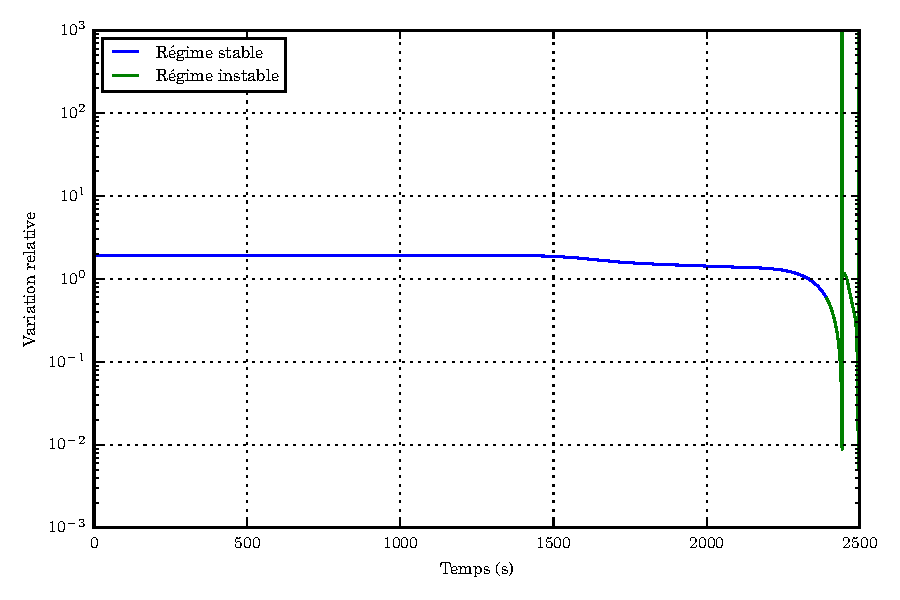
\includegraphics{figures/df_dS_and_df_dT.pdf}
  \caption{Variation du rapport $\Delta T \frac{\mathrm{d} f}{\mathrm d T}$ sur $\Delta S \frac{\mathrm{d} f}{\mathrm d S}$ au cours de la simulation. En bleu, le régime stable (utilisation d'un schéma implicite pour $S$) et en vert le régime instable (utilisation d'un schéma explicite pour $S$). On constate que dans le régime stable, la variation du terme de chauffage par une perturbation en température est plus grande que la variation par une perturbation en densité surfacique. Le rapport devient très variable lorsque le disque devient instable.}
  \label{fig:df_ds_et_df_dt}
\end{figure}

%%% Local Variables:
%%% mode: latex
%%% TeX-master: "rapport"
%%% End:
